\documentclass{article}

\usepackage{graphicx}
\usepackage{tikz}
\usepackage{tikzsymbols}
\usetikzlibrary{calc,patterns,shapes.geometric}
\pagestyle{empty}
\usepackage[margin=0pt]{geometry}
\geometry{papersize={14in,12in}}

\def\centerarc[#1](#2)(#3:#4:#5){\draw[#1] ($(#2)+({#5*cos(#3)},{#5*sin(#3)})$) arc (#3:#4:#5);}

\begin{document}
	\begin{figure}
		\centering
		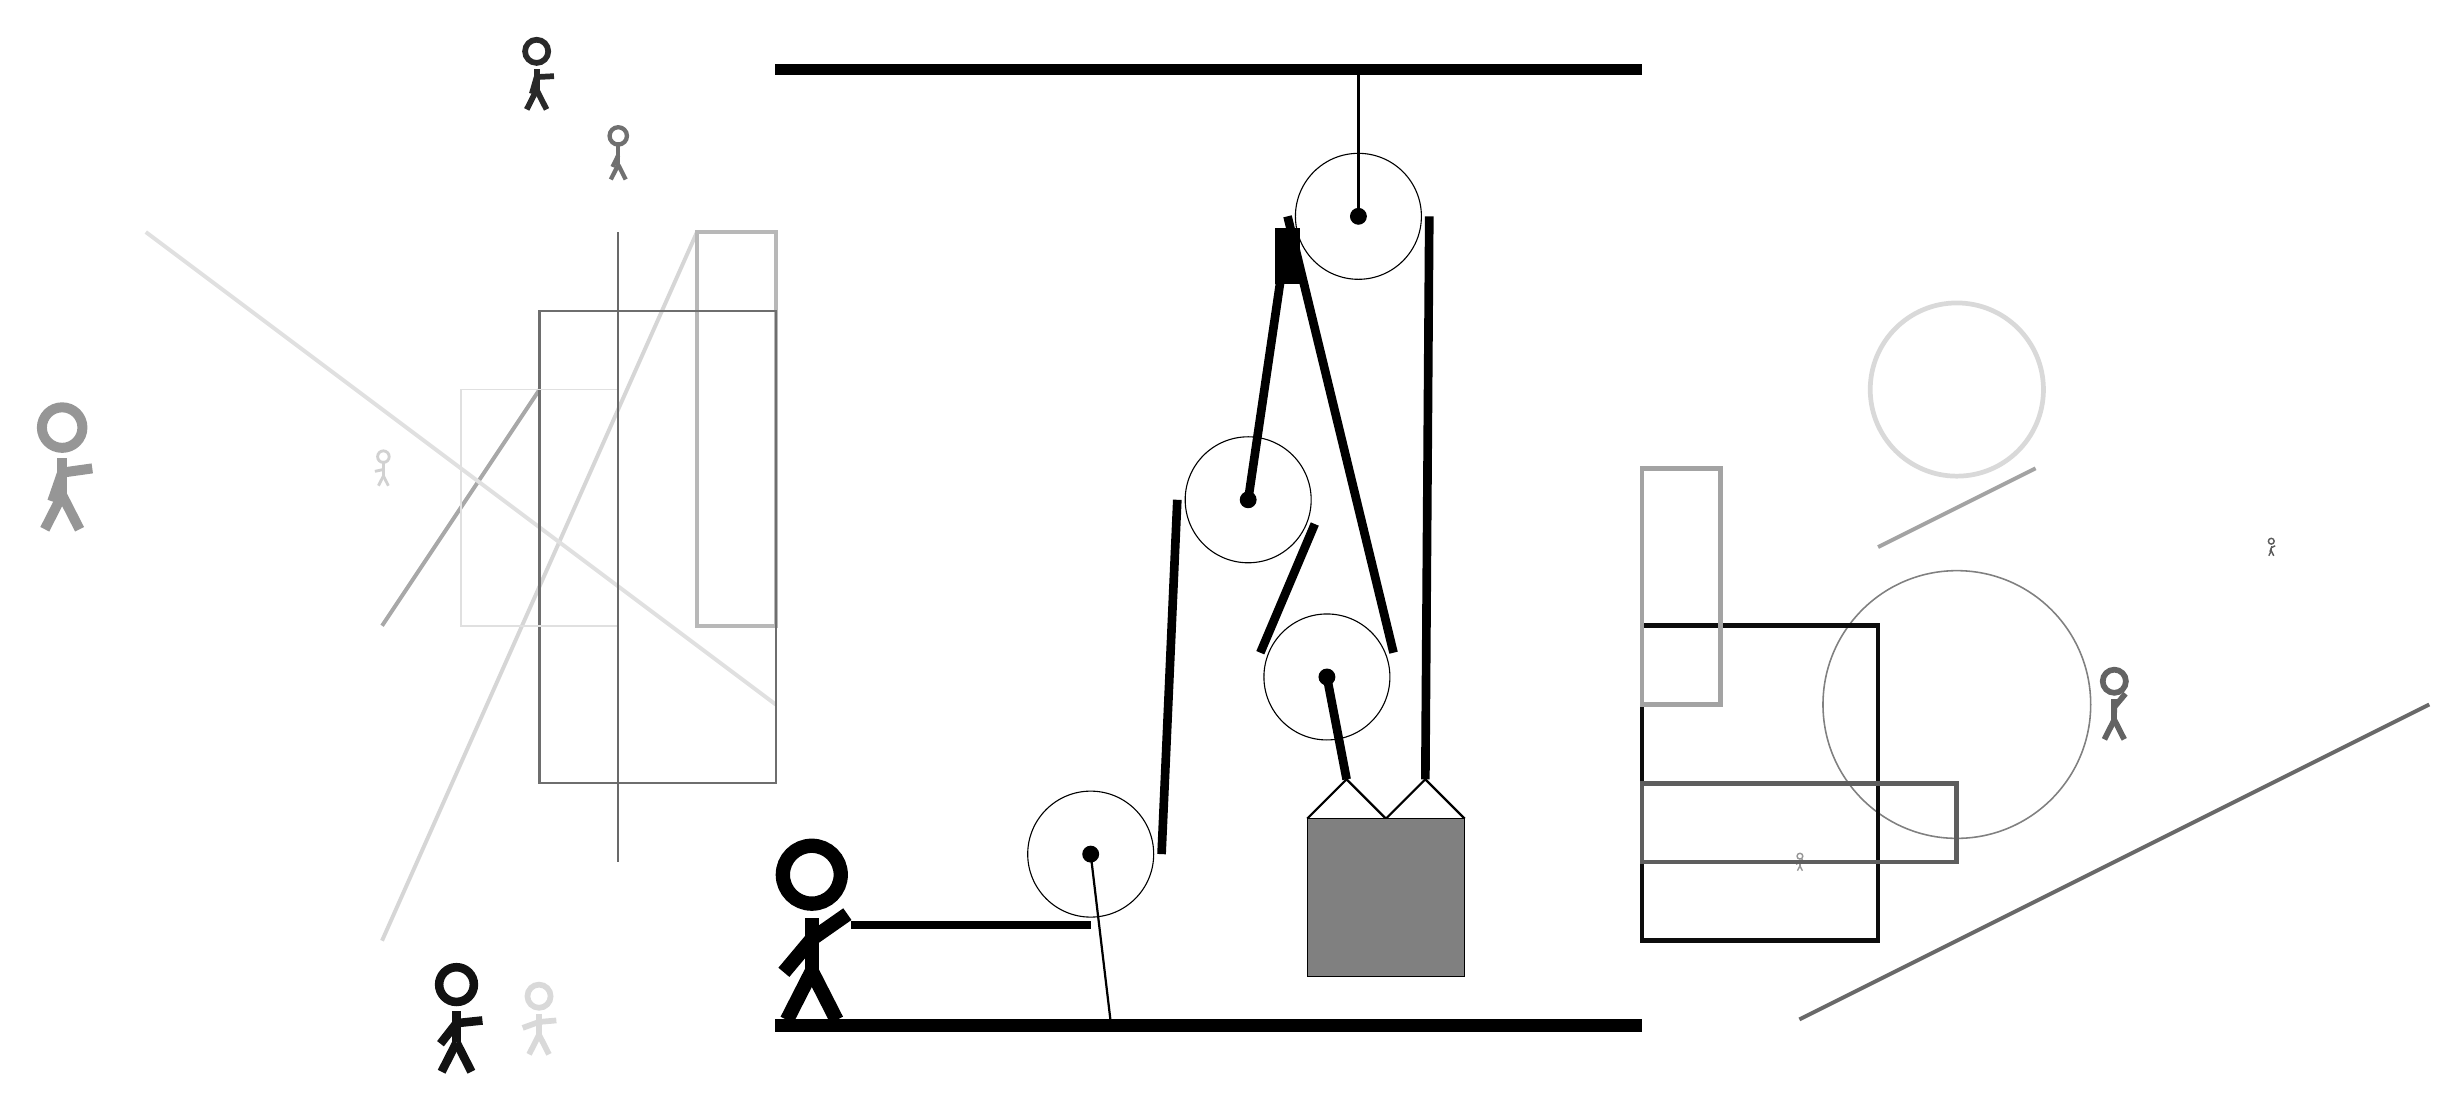
\begin{tikzpicture}
			%%%%% START %%%%%
			
			\draw[fill=black] (-6, 9) rectangle (5, 9.125);
			
			\node[line width=0.3mm, color=black!41] at (7, -1) {\Strichmaxerl[1][22][54]};
			
			\node[line width=0.5mm, color=black!61] at (11, 1) {\Strichmaxerl[4][88][50]};
			\draw[line width=0.5mm, color=black!36](8, 3) -- (10, 4);
			\draw [line width=0.2mm, color=black!50](9, 1) circle (1.7);
			
			\node[line width=0.5mm, color=black!56] at (-8, 8) {\Strichmaxerl[3][64][90]};
			
			\node[line width=0.5mm, color=black!84] at (-9, 9) {\Strichmaxerl[4][74][3]};
			
			\node[line width=0.2mm, color=black!93] at (-10, -3) {\Strichmaxerl[6][52][6]};
			
			\draw[line width=0.5mm, color=black!16](-11, -2) -- (-7, 7);
			\draw[line width=0.6mm, color=black!95] (5, 2) rectangle (8, -2);
			\draw[line width=0.5mm, color=black!34](-9, 5) -- (-11, 2);
			\node[line width=0.7mm, color=black!15] at (-9, -3) {\Strichmaxerl[4][20][5]};
			\draw[line width=0.5mm, color=black!28] (-7, 2) rectangle (-6, 7);
			\draw[line width=0.5mm, color=black!59](7, -3) -- (15, 1);
			
			\draw[line width=0.5mm, color=black!12](-6, 1) -- (-14, 7);
			\draw[line width=0.6mm, color=black!36] (5, 1) rectangle (6, 4);
			\node[line width=0.2mm, color=black!64] at (13, 3) {\Strichmaxerl[1][72][25]};
			
			\node[line width=0.2mm, color=black!18] at (-11, 4) {\Strichmaxerl[2][12][89]};
			\draw[line width=0.3mm, color=black!57] (-6, 6) rectangle (-9, 0);
			\node[line width=0.6mm, color=black!41] at (-15, 4) {\Strichmaxerl[7][71][8]};
			\draw[line width=0.2mm, color=black!12] (-8, 2) rectangle (-10, 5);
			\draw[line width=0.3mm, color=black!59] (-8, 7) rectangle (-8, -1);
			
			\draw[line width=0.6mm, color=black!63] (5, -1) rectangle (9, 0);
			
			\draw [line width=0.6mm, color=black!15](9, 5) circle (1.1);
			
			\draw (0, 3.6) circle (0.8);
			\draw[fill=black] (0, 3.6) circle (0.1);
			
			\draw (1, 1.35) circle (0.8);
			\draw[fill=black] (1, 1.35) circle (0.1);
			
			\draw (1.4, 7.2) circle (0.8);
			\draw[fill=black] (1.4, 7.2) circle (0.1);
			\draw[very thick] (1.4, 7.2) -- (1.4, 9);
			
			\draw (-2, -0.9) circle (0.8);
			\draw[fill=black] (-2, -0.9) circle (0.1);
			\draw[thick] (-2, -0.9) -- (-1.75, -3);
			
			
			\draw[thick]  (0.75, -0.45) -- (1.25, 0.05) -- (1.75, -0.45) -- (2.25, 0.05) -- (2.75, -0.45);
			\draw[fill=black!50] (0.75, -0.45) rectangle (2.75, -2.45);
			\draw[line width=1.1mm] (-5.05, -1.8) -- (-2, -1.8);
			\centerarc[line width=1.1mm](-2, -0.9)(270:360:0.9);
			\draw[line width=1.1mm] (-1.1, -0.9) -- (-0.9, 3.6);
			\draw[line width=1.1mm] (0, 3.6) -- (0.5, 7.0);
			\draw[line width=1.1mm, fill=black](0.4, 6.4) rectangle (0.6, 7.0);
			\centerarc[line width=1.1mm](0, 3.6)(-20:180:0.9);
			\draw[line width=1.1mm] (0.8457, 3.2922) -- (0.1543, 1.6578);
			\centerarc[line width=1.1mm](1, 1.35)(160:380:0.9);
			\draw[line width=1.1mm] (1.8457, 1.6578) -- (0.5, 7.2);
			\draw[line width=1.1mm](1, 1.35) -- (1.25, 0.05);
			\centerarc[line width=1.1mm](1.4, 7.2)(0:180:0.9);
			\draw[line width=1.1mm] (2.3, 7.2) -- (2.25, 0.05);
			
			\node at (-5.5, -1.9) {\Strichmaxerl[10][50][35]};
			
			\draw[fill=black] (-6, -3) rectangle (5, -3.15);
			
			%%%%% END %%%%%
		\end{tikzpicture}
	\end{figure}	
\end{document}